%----------------------------------------------------------------------------------------
%	PACKAGES AND OTHER DOCUMENT CONFIGURATIONS
%----------------------------------------------------------------------------------------

\documentclass[11pt,fleqn]{book} % Default font size and left-justified equations

\usepackage[top=3cm,bottom=3cm,left=3.2cm,right=3.2cm,headsep=10pt,letterpaper]{geometry} % Page margins

\usepackage{xcolor} % Required for specifying colors by name
\definecolor{ocre}{RGB}{52,177,201} % Define the orange color used for highlighting throughout the book

% Font Settings
\usepackage{avant} % Use the Avantgarde font for headings
%\usepackage{times} % Use the Times font for headings
\usepackage{mathptmx} % Use the Adobe Times Roman as the default text font together with math symbols from the Sym­bol, Chancery and Com­puter Modern fonts

\usepackage{microtype} % Slightly tweak font spacing for aesthetics
\usepackage[utf8]{inputenc} % Required for including letters with accents
\usepackage[T1]{fontenc} % Use 8-bit encoding that has 256 glyphs

\usepackage{type1cm}
\usepackage{lettrine}

% Bibliography
\usepackage[style=alphabetic,sorting=nyt,sortcites=true,autopunct=true,babel=hyphen,hyperref=true,abbreviate=false,backref=true,backend=biber]{biblatex}
\addbibresource{bibliography.bib} % BibTeX bibliography file
\defbibheading{bibempty}{}

%%%%%%%%%%%%%%%%%%%%%%%%%%%%%%%%%%%%%%%%%
% This is based on the Legrand Orange Book
% Structural Definitions File
%
% The original template (the Legrand Orange Book Template) can be found here --> http://www.latextemplates.com/template/the-legrand-orange-book
%
% Original author of the Legrand Orange Book Template::
% Mathias Legrand (legrand.mathias@gmail.com) with modifications by:
% Vel (vel@latextemplates.com)
%
% Original License:
% CC BY-NC-SA 3.0 (http://creativecommons.org/licenses/by-nc-sa/3.0/)
%
%%%%%%%%%%%%%%%%%%%%%%%%%%%%%%%%%%%%%%%%%
%----------------------------------------------------------------------------------------
%	VARIOUS REQUIRED PACKAGES
%----------------------------------------------------------------------------------------

\usepackage{titlesec} % Allows customization of titles

\usepackage{graphicx} % Required for including pictures
\graphicspath{{Pictures/}} % Specifies the directory where pictures are stored

\usepackage{lipsum} % Inserts dummy text

\usepackage{tikz} % Required for drawing custom shapes

\usepackage[english]{babel} % English language/hyphenation

\usepackage{enumitem} % Customize lists
\setlist{nolistsep} % Reduce spacing between bullet points and numbered lists

\usepackage{booktabs} % Required for nicer horizontal rules in tables

\usepackage{eso-pic} % Required for specifying an image background in the title page

%----------------------------------------------------------------------------------------
%	MAIN TABLE OF CONTENTS
%----------------------------------------------------------------------------------------

\usepackage{titletoc} % Required for manipulating the table of contents

\contentsmargin{0cm} % Removes the default margin
% Chapter text styling
\titlecontents{chapter}[1.25cm] % Indentation
{\addvspace{15pt}\large\sffamily\bfseries} % Spacing and font options for chapters
{\color{ocre!60}\contentslabel[\Large\thecontentslabel]{1.25cm}\color{ocre}} % Chapter number
{}  
{\color{ocre!60}\normalsize\sffamily\bfseries\;\titlerule*[.5pc]{.}\;\thecontentspage} % Page number
% Section text styling
\titlecontents{section}[1.25cm] % Indentation
{\addvspace{5pt}\sffamily\bfseries} % Spacing and font options for sections
{\contentslabel[\thecontentslabel]{1.25cm}} % Section number
{}
{\sffamily\hfill\color{black}\thecontentspage} % Page number
[]
% Subsection text styling
\titlecontents{subsection}[1.25cm] % Indentation
{\addvspace{1pt}\sffamily\small} % Spacing and font options for subsections
{\contentslabel[\thecontentslabel]{1.25cm}} % Subsection number
{}
{\sffamily\;\titlerule*[.5pc]{.}\;\thecontentspage} % Page number
[] 

%----------------------------------------------------------------------------------------
%	MINI TABLE OF CONTENTS IN CHAPTER HEADS
%----------------------------------------------------------------------------------------

% Section text styling
\titlecontents{lsection}[0em] % Indendating
{\footnotesize\sffamily} % Font settings
{}
{}
{}

% Subsection text styling
\titlecontents{lsubsection}[.5em] % Indentation
{\normalfont\footnotesize\sffamily} % Font settings
{}
{}
{}
 
%----------------------------------------------------------------------------------------
%	PAGE HEADERS
%----------------------------------------------------------------------------------------

\usepackage{fancyhdr} % Required for header and footer configuration

\pagestyle{fancy}
\renewcommand{\chaptermark}[1]{\markboth{\sffamily\normalsize\bfseries\chaptername\ \thechapter.\ #1}{}} % Chapter text font settings
\renewcommand{\sectionmark}[1]{\markright{\sffamily\normalsize\thesection\hspace{5pt}#1}{}} % Section text font settings
\fancyhf{} \fancyhead[LE,RO]{\sffamily\normalsize\thepage} % Font setting for the page number in the header
\fancyhead[LO]{\rightmark} % Print the nearest section name on the left side of odd pages
\fancyhead[RE]{\leftmark} % Print the current chapter name on the right side of even pages
\renewcommand{\headrulewidth}{0.5pt} % Width of the rule under the header
\addtolength{\headheight}{2.5pt} % Increase the spacing around the header slightly
\renewcommand{\footrulewidth}{0pt} % Removes the rule in the footer
\fancypagestyle{plain}{\fancyhead{}\renewcommand{\headrulewidth}{0pt}} % Style for when a plain pagestyle is specified

% Removes the header from odd empty pages at the end of chapters
\makeatletter
\renewcommand{\cleardoublepage}{
\clearpage\ifodd\c@page\else
\hbox{}
\vspace*{\fill}
\thispagestyle{empty}
\newpage
\fi}

%----------------------------------------------------------------------------------------
%	THEOREM STYLES
%----------------------------------------------------------------------------------------

\usepackage{amsmath,amsfonts,amssymb,amsthm} % For math equations, theorems, symbols, etc

\newcommand{\intoo}[2]{\mathopen{]}#1\,;#2\mathclose{[}}
\newcommand{\ud}{\mathop{\mathrm{{}d}}\mathopen{}}
\newcommand{\intff}[2]{\mathopen{[}#1\,;#2\mathclose{]}}
\newtheorem{notation}{Notation}[chapter]

%%%%%%%%%%%%%%%%%%%%%%%%%%%%%%%%%%%%%%%%%%%%%%%%%%%%%%%%%%%%%%%%%%%%%%%%%%%
%%%%%%%%%%%%%%%%%%%% dedicated to boxed/framed environements %%%%%%%%%%%%%%
%%%%%%%%%%%%%%%%%%%%%%%%%%%%%%%%%%%%%%%%%%%%%%%%%%%%%%%%%%%%%%%%%%%%%%%%%%%
\newtheoremstyle{ocrenumbox}% % Theorem style name
{0pt}% Space above
{0pt}% Space below
{\normalfont}% % Body font
{}% Indent amount
{\small\bf\sffamily\color{ocre}}% % Theorem head font
{\;}% Punctuation after theorem head
{0.25em}% Space after theorem head
{\small\sffamily\color{ocre}\thmname{#1}\nobreakspace\thmnumber{\@ifnotempty{#1}{}\@upn{#2}}% Theorem text (e.g. Theorem 2.1)
\thmnote{\nobreakspace\the\thm@notefont\sffamily\bfseries\color{black}---\nobreakspace#3.}} % Optional theorem note
\renewcommand{\qedsymbol}{$\blacksquare$}% Optional qed square

\newtheoremstyle{blacknumex}% Theorem style name
{5pt}% Space above
{5pt}% Space below
{\normalfont}% Body font
{} % Indent amount
{\small\bf\sffamily}% Theorem head font
{\;}% Punctuation after theorem head
{0.25em}% Space after theorem head
{\small\sffamily{\tiny\ensuremath{\blacksquare}}\nobreakspace\thmname{#1}\nobreakspace\thmnumber{\@ifnotempty{#1}{}\@upn{#2}}% Theorem text (e.g. Theorem 2.1)
\thmnote{\nobreakspace\the\thm@notefont\sffamily\bfseries---\nobreakspace#3.}}% Optional theorem note

\newtheoremstyle{blacknumbox} % Theorem style name
{0pt}% Space above
{0pt}% Space below
{\normalfont}% Body font
{}% Indent amount
{\small\bf\sffamily}% Theorem head font
{\;}% Punctuation after theorem head
{0.25em}% Space after theorem head
{\small\sffamily\thmname{#1}\nobreakspace\thmnumber{\@ifnotempty{#1}{}\@upn{#2}}% Theorem text (e.g. Theorem 2.1)
\thmnote{\nobreakspace\the\thm@notefont\sffamily\bfseries---\nobreakspace#3.}}% Optional theorem note

%%%%%%%%%%%%%%%%%%%%%%%%%%%%%%%%%%%%%%%%%%%%%%%%%%%%%%%%%%%%%%%%%%%%%%%%%%%
%%%%%%%%%%%%% dedicated to non-boxed/non-framed environements %%%%%%%%%%%%%
%%%%%%%%%%%%%%%%%%%%%%%%%%%%%%%%%%%%%%%%%%%%%%%%%%%%%%%%%%%%%%%%%%%%%%%%%%%
\newtheoremstyle{ocrenum}% % Theorem style name
{5pt}% Space above
{5pt}% Space below
{\normalfont}% % Body font
{}% Indent amount
{\small\bf\sffamily\color{ocre}}% % Theorem head font
{\;}% Punctuation after theorem head
{0.25em}% Space after theorem head
{\small\sffamily\color{ocre}\thmname{#1}\nobreakspace\thmnumber{\@ifnotempty{#1}{}\@upn{#2}}% Theorem text (e.g. Theorem 2.1)
\thmnote{\nobreakspace\the\thm@notefont\sffamily\bfseries\color{black}---\nobreakspace#3.}} % Optional theorem note
\renewcommand{\qedsymbol}{$\blacksquare$}% Optional qed square
\makeatother

% Defines the theorem text style for each type of theorem to one of the three styles above
\newcounter{dummy} 
\numberwithin{dummy}{section}
\theoremstyle{ocrenumbox}
\newtheorem{theoremeT}[dummy]{Theorem}
\newtheorem{problem}{Problem}[chapter]
\newtheorem{exerciseT}{Exercise}[chapter]
\theoremstyle{blacknumex}
\newtheorem{exampleT}{Example}[chapter]
\theoremstyle{blacknumbox}
\newtheorem{vocabulary}{Vocabulary}[chapter]
\newtheorem{definitionT}{Definition}[section]
\newtheorem{corollaryT}[dummy]{Corollary}
\theoremstyle{ocrenum}
\newtheorem{proposition}[dummy]{Proposition}

%----------------------------------------------------------------------------------------
%	DEFINITION OF COLORED BOXES
%----------------------------------------------------------------------------------------

\RequirePackage[framemethod=default]{mdframed} % Required for creating the theorem, definition, exercise and corollary boxes

% Theorem box
\newmdenv[skipabove=7pt,
skipbelow=7pt,
backgroundcolor=black!5,
linecolor=ocre,
innerleftmargin=5pt,
innerrightmargin=5pt,
innertopmargin=5pt,
leftmargin=0cm,
rightmargin=0cm,
innerbottommargin=5pt]{tBox}

% Exercise box	  
\newmdenv[skipabove=7pt,
skipbelow=7pt,
rightline=false,
leftline=true,
topline=false,
bottomline=false,
backgroundcolor=ocre!10,
linecolor=ocre,
innerleftmargin=5pt,
innerrightmargin=5pt,
innertopmargin=5pt,
innerbottommargin=5pt,
leftmargin=0cm,
rightmargin=0cm,
linewidth=4pt]{eBox}	

% Definition box
\newmdenv[skipabove=7pt,
skipbelow=7pt,
rightline=false,
leftline=true,
topline=false,
bottomline=false,
linecolor=ocre,
innerleftmargin=5pt,
innerrightmargin=5pt,
innertopmargin=0pt,
leftmargin=0cm,
rightmargin=0cm,
linewidth=4pt,
innerbottommargin=0pt]{dBox}	

% Corollary box
\newmdenv[skipabove=7pt,
skipbelow=7pt,
rightline=false,
leftline=true,
topline=false,
bottomline=false,
linecolor=gray,
backgroundcolor=black!5,
innerleftmargin=5pt,
innerrightmargin=5pt,
innertopmargin=5pt,
leftmargin=0cm,
rightmargin=0cm,
linewidth=4pt,
innerbottommargin=5pt]{cBox}

% Creates an environment for each type of theorem and assigns it a theorem text style from the "Theorem Styles" section above and a colored box from above
\newenvironment{theorem}{\begin{tBox}\begin{theoremeT}}{\end{theoremeT}\end{tBox}}
\newenvironment{exercise}{\begin{eBox}\begin{exerciseT}}{\hfill{\color{ocre}\tiny\ensuremath{\blacksquare}}\end{exerciseT}\end{eBox}}				  
\newenvironment{definition}{\begin{dBox}\begin{definitionT}}{\end{definitionT}\end{dBox}}	
\newenvironment{example}{\begin{exampleT}}{\hfill{\tiny\ensuremath{\blacksquare}}\end{exampleT}}		
\newenvironment{corollary}{\begin{cBox}\begin{corollaryT}}{\end{corollaryT}\end{cBox}}	

%----------------------------------------------------------------------------------------
%	REMARK ENVIRONMENT
%----------------------------------------------------------------------------------------

\newenvironment{remark}{\par\vspace{10pt}\small % Vertical white space above the remark and smaller font size
\begin{list}{}{
\leftmargin=35pt % Indentation on the left
\rightmargin=25pt}\item\ignorespaces % Indentation on the right
\makebox[-2.5pt]{\begin{tikzpicture}[overlay]
\node[draw=ocre!60,line width=1pt,circle,fill=ocre!25,font=\sffamily\bfseries,inner sep=2pt,outer sep=0pt] at (-15pt,0pt){\textcolor{ocre}{R}};\end{tikzpicture}} % Orange R in a circle
\advance\baselineskip -1pt}{\end{list}\vskip5pt} % Tighter line spacing and white space after remark

%----------------------------------------------------------------------------------------
%	SECTION NUMBERING IN THE MARGIN
%----------------------------------------------------------------------------------------

\makeatletter
\renewcommand{\@seccntformat}[1]{\llap{\textcolor{ocre}{\csname the#1\endcsname}\hspace{1em}}}                    
\renewcommand{\section}{\@startsection{section}{1}{\z@}
{-4ex \@plus -1ex \@minus -.4ex}
{1ex \@plus.2ex }
{\normalfont\large\sffamily\bfseries}}
\renewcommand{\subsection}{\@startsection {subsection}{2}{\z@}
{-3ex \@plus -0.1ex \@minus -.4ex}
{0.5ex \@plus.2ex }
{\normalfont\sffamily\bfseries}}
\renewcommand{\subsubsection}{\@startsection {subsubsection}{3}{\z@}
{-2ex \@plus -0.1ex \@minus -.2ex}
{.2ex \@plus.2ex }
{\normalfont\small\sffamily\bfseries}}                        
\renewcommand\paragraph{\@startsection{paragraph}{4}{\z@}
{-2ex \@plus-.2ex \@minus .2ex}
{.1ex}
{\normalfont\small\sffamily\bfseries}}

%----------------------------------------------------------------------------------------
%	HYPERLINKS IN THE DOCUMENTS
%----------------------------------------------------------------------------------------

% For an unclear reason, the package should be loaded now and not later
\usepackage{hyperref}
\hypersetup{hidelinks,backref=true,pagebackref=true,hyperindex=true,colorlinks=false,breaklinks=true,urlcolor= ocre,bookmarks=true,bookmarksopen=false,pdftitle={Title},pdfauthor={Author}}

%----------------------------------------------------------------------------------------
%	CHAPTER HEADINGS
%----------------------------------------------------------------------------------------

% The set-up below should be (sadly) manually adapted to the overall margin page septup controlled by the geometry package loaded in the main.tex document. It is possible to implement below the dimensions used in the goemetry package (top,bottom,left,right)... TO BE DONE

\newcommand{\thechapterimage}{}
\newcommand{\chapterimage}[1]{\renewcommand{\thechapterimage}{#1}}

% Numbered chapters with mini tableofcontents
\def\thechapter{\arabic{chapter}}
\def\@makechapterhead#1{
\thispagestyle{empty}
{\centering \normalfont\sffamily
\ifnum \c@secnumdepth >\m@ne
\if@mainmatter
\startcontents
\begin{tikzpicture}[remember picture,overlay]
\node at (current page.north west)
{\begin{tikzpicture}[remember picture,overlay]
\node[anchor=north west,inner sep=0pt] at (0,0) {\includegraphics[width=\paperwidth]{\thechapterimage}};
%%%%%%%%%%%%%%%%%%%%%%%%%%%%%%%%%%%%%%%%%%%%%%%%%%%%%%%%%%%%%%%%%%%%%%%%%%%%%%%%%%%%%
% Commenting the 3 lines below removes the small contents box in the chapter heading
%\fill[color=ocre!10!white,opacity=.6] (1cm,0) rectangle (8cm,-7cm);
%\node[anchor=north west] at (1.1cm,.35cm) {\parbox[t][8cm][t]{6.5cm}{\huge\bfseries\flushleft \printcontents{l}{1}{\setcounter{tocdepth}{2}}}};
\draw[anchor=west] (5cm,-9cm) node [rounded corners=20pt,fill=ocre!10!white,text opacity=1,draw=ocre,draw opacity=1,line width=1.5pt,fill opacity=.6,inner sep=12pt]{\huge\sffamily\bfseries\textcolor{black}{\thechapter. #1\strut\makebox[22cm]{}}};
%%%%%%%%%%%%%%%%%%%%%%%%%%%%%%%%%%%%%%%%%%%%%%%%%%%%%%%%%%%%%%%%%%%%%%%%%%%%%%%%%%%%%
\end{tikzpicture}};
\end{tikzpicture}}
\par\vspace*{230\p@}
\fi
\fi}

% Unnumbered chapters without mini tableofcontents (could be added though) 
\def\@makeschapterhead#1{
\thispagestyle{empty}
{\centering \normalfont\sffamily
\ifnum \c@secnumdepth >\m@ne
\if@mainmatter
\begin{tikzpicture}[remember picture,overlay]
\node at (current page.north west)
{\begin{tikzpicture}[remember picture,overlay]
\node[anchor=north west,inner sep=0pt] at (0,0) {\includegraphics[width=\paperwidth]{\thechapterimage}};
\draw[anchor=west] (5cm,-9cm) node [rounded corners=20pt,fill=ocre!10!white,fill opacity=.6,inner sep=12pt,text opacity=1,draw=ocre,draw opacity=1,line width=1.5pt]{\huge\sffamily\bfseries\textcolor{black}{#1\strut\makebox[22cm]{}}};
\end{tikzpicture}};
\end{tikzpicture}}
\par\vspace*{230\p@}
\fi
\fi
}
\makeatother % Insert the commands.tex file which contains the majority of the structure behind the template


%\documentclass[twoside]{article}
\usepackage{lipsum} % for filler text
\usepackage{fancyhdr}
\pagestyle{fancy}
\pagenumbering{arabic}
\fancyhead{} % clear all header fields
\renewcommand{\headrulewidth}{0pt} % no line in header area
\fancyfoot{} % clear all footer fields
\fancyfoot[LE,RO]{\thepage}           % page number in "outer" position of footer line
\fancyfoot[RE,LO]{SVPM's CoE Malegaon(Bk.), Dept. of Computer Engg.(2018-19)} % other info in "inner" position of footer line

\begin{document}
\title{Smart Real Estate Assessment}

%----------------------------------------------------------------------------------------
%	TITLE PAGE
%----------------------------------------------------------------------------------------

\begingroup
\thispagestyle{empty}
\AddToShipoutPicture*{\put(0,0){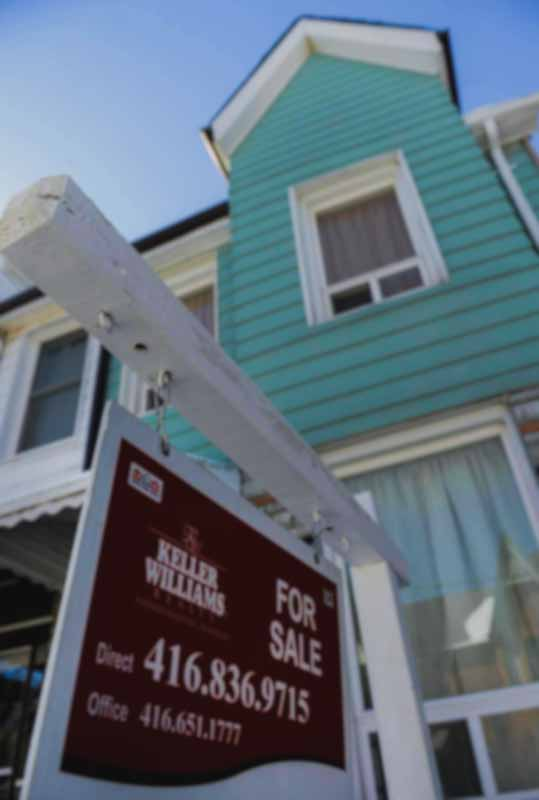
\includegraphics[scale=1.25]{front.jpg}}} % Image background
\centering
\vspace*{1cm}
\par\normalfont\fontsize{40}{35}\sffamily\selectfont\color{white}
{\LARGE A Preliminary Project Report on}\par 
\vspace*{4cm}
\textbf{SMART REAL ESTATE ASSESSMENT}\\ % Project title
\vspace*{4cm}
{\large Presented By}\par
\vspace*{1cm}
{\Huge Patne Nikhil}\par
{\Huge Shinde Abhishek}\par
{\Huge Gholap Satyawan}\par
{\Huge Dange Namrata}\par
{\Huge Beera Vivechana}\par
\endgroup

%----------------------------------------------------------------------------------------
%	COPYRIGHT PAGE
%----------------------------------------------------------------------------------------

\newpage
~\vfill
\thispagestyle{empty}
\vspace{-5cm}
\begin{center}
	  \begin{figure}[h]
			\centering
			
\includegraphics[width=5 cm]{Pictures/coem.png}
		\end{figure}
	  \fontsize{10}{10}\textbf{\LARGE DEPARTMENT OF COMPUTER ENGINEERING}\\
	  SVPM'S COLLEGE OF ENGINEERING\\
	  MALEGAON(Bk) \\
	   2018-19
	  \end{center}
	 \vspace{0cm}
\begin{center}
\text{\LARGE Sponsored by}
	  \begin{figure}[h]
			\centering
			
\includegraphics[width=5 cm]{Pictures/xento_logo_1200X630.jpg}
		\end{figure}
	  \end{center}
	  \begin{center}
	      \text{Xento Systems Private Limited, Pune}
	  \end{center}
\vspace{2cm}
%\noindent Copyright \copyright\ 2014 Andrea Hidalgo\\ % Copyright notice

\noindent \textsc{SVPM's College of Engineering Malegaon(Bk.) Baramati}\\
\noindent \textsc{github.com/AbhieShinde/Project}\\ % URL
\noindent This research was done under the guidance of Prof. Nimbalkar S.S. and Prof. Khumbhar H.R. with in the sponsorship of Xento Systems Pvt. Ltd., Pune, from August 2018.\\ % License information

%----------------------------------------------------------------------------------------
%	CERTIFICATE
%----------------------------------------------------------------------------------------
\newpage


\begin{figure}[ht]
\centering

\includegraphics[scale=0.4]{Pictures/coem.png}
\end{figure}


{\bfseries \fontsize{14}{12} \selectfont \centerline{SVPM's COLLEGE OF ENGINEERING}
\centerline{DEPARTMENT OF COMPUTER ENGINEERING}
\vspace*{1.2\baselineskip}} 


{\bfseries \fontsize{20}{20} \selectfont \centerline{\color{ocre} CERTIFICATE} 
\vspace*{1.4\baselineskip}} 

\centerline{This is to certify that the Project Entitled}
\vspace*{1\baselineskip} 


{\bfseries \fontsize{20}{12} \selectfont \centerline{\color{ocre}\LARGE Smart Real Estate Assessment}
\vspace*{1\baselineskip}}

\centerline{Submitted by}
\vspace*{0.72\baselineskip} 
\centerline{\LARGE Dange Namrata Milind \hspace{25 mm} Exam No:B150194\textbf{\color{ocre}206}}
\vspace{2mm}
\centerline{\LARGE Gholap Satywan Ashok \hspace{24 mm} Exam No:B150194\textbf{\color{ocre}214}}
\vspace{2mm}
\centerline{\LARGE Patne Nikhil Sunil \hspace{37 mm} Exam No:B150194\textbf{\color{ocre}234}}
\vspace{2mm}
\centerline{\LARGE Shinde Abhishek Sunil \hspace{26 mm} Exam No:B150194\textbf{\color{ocre}242}}
\vspace{2mm}
\centerline{\LARGE Beera Vivechana Ramesh \hspace{20 mm} Exam No:B150194\textbf{\color{ocre}259}}
\vspace*{1\baselineskip} 
is a bonafide work carried out by Students under the supervision of\\ \textbf{\LARGE\color{ocre} Prof. Nimbalkar S.S.} and it
is submitted towards the partial fulfillment of the requirement of Bachelor of Engineering (Computer Engineering) Project.\\[1cm]

\bgroup
\def\arraystretch{0.7}
\begin{tabular}{c c }
\vspace{2mm}
Prof.Nimbalkar S.S &  \hspace{40 mm} Prof.Kumbhar H.R \\								
\vspace{2mm}
Internal Guide   &  \hspace{40 mm} H.O.D \\[2cm]
\vspace{0.1cm}\_\_\_\_\_\_\_\_\_\_\_\_\_\_\_\_\_\_\_\_\_\_\_\_ & \hspace{40 mm} \_\_\_\_\_\_\_\_\_\_\_\_\_\_\_\_\_\_\_\_\_\_\_\_\\
External Examiner &\hspace{40 mm}Principal\\
\end{tabular}\\[1cm]
Place : SVPM's COE Malegaon(Bk.)\\
Date  : 


%----------------------------------------------------------------------------------------
%	Acknowledgments
%----------------------------------------------------------------------------------------
%\lipsum[1-20]
\newpage
\bfseries \fontsize{15}{19} \normalfont \centerline{\LARGE\color{ocre} Acknowledgments} 
			          \pagestyle{empty}
			         {\setlength{\baselineskip}{2\baselineskip}}
			         
\textit{It gives us great pleasure in presenting the preliminary project report 
on {\bfseries \fontsize{12}{12} \color{ocre} `Smart Real Estate Assessment'}.}
\vspace*{1.5\baselineskip}

 \textit{I would like to take this opportunity to thank my internal guide
 \textbf{Prof. Nimbalkar S.S}  and all teachers for giving me all the help and guidance I needed. I am
 really grateful to them for their kind support.I appreciate all valuable suggestions given  and queries raised by her which really helped us in exploring project in deep.} \vspace*{1.5\baselineskip}

 \textit{I am also grateful to \textbf{\color{ocre}Prof.Kumbhar H.R}, Head of Computer
 Engineering Department, SVPM COE for his indispensable
 support, suggestions.}
\vspace*{1.5\baselineskip}

\textit{In the end our special thanks to \textbf{\color{ocre}Mr.Nimbalkar S.S} for
providing various resources such as  laboratory with all needed software platforms,
continuous Internet connection, for Our Project.}
\vspace*{3\baselineskip} \\

\begin{flushright}
\begin{tabular}{p{8.2cm}c}
&\hspace{6 mm}Dange Namrata\\
&\hspace{8 mm}Gholap Satywan\\
&Patne Nikhil\\
&\hspace{9mm}Shinde Abhishek\\
&\hspace{9mm}Beera Vivechana\\[1cm]
&\hspace{7 mm}(B.E. Computer Engg.)

\end{tabular}
\end{flushright}

\maketitle
\addcontentsline{toc}{section}{Acknowledgment}


\newpage
\bfseries \fontsize{15}{19} \normalfont \centerline{\LARGE\color{ocre} Abstract} 
			          \pagestyle{empty}
			         {\setlength{\baselineskip}{1\baselineskip}
			         
\paragraph*{}\lettrine[lines=2]{\color{ocre!60} R}{eal} estate appraisal, which is the process of estimating the price for real estate properties, is crucial for both buys and sellers as the basis for negotiation and transaction. Traditionally, the repeat sales model has been widely adopted to estimate real estate price. However, it depends the design and calculation of a complex economic related index, which is challenging to estimate accurately. Today, real estate brokers provide easy access to detailed online information on real estate properties to their clients. We are interested in estimating the real estate price from these large amounts of easily accessed data. In particular, we analyze the prediction power of online house pictures, which is one of the key factors for online users to make a potential visiting decision. The development of robust computer vision algorithms makes the analysis of visual content possible. In this work, we employ a Recurrent Neural Network (RNN) to predict real estate price using the state-of-the-art visual features.\\
In a smart city, effective and accurate real estate assessments governed by a local government is crucial for determining the property taxes. Such assessments have never been trivial, and inappropriate assessments may result in disputes between property owners and the local government.\\
Generally for price prediction \textbf{\color{ocre} Regression} is used (Prediction of continuos valued-function). But here we are going to use \textbf{\color{ocre} Structured Deep Neural Network} in order to improve efficiency and accuracy. We introduce a deep learning approach to smartly and effectively assessing real estate values. We propose a systematic method to derive a layered knowledge graph and design a structured Deep Neural Network (DNN) based on it. Neurons in a structured DNN are structurally connected, which makes the network time and space efficient; and thus, it requires fewer data points for training. The structured DNN model has been designed to learn from the most recently captured data points; therefore, it allows the model to adapt to the latest market trends.

 \addcontentsline{toc}{section}{Abstract}
			         }


%----------------------------------------------------------------------------------------
%	TABLE OF CONTENTS
%----------------------------------------------------------------------------------------

\chapterimage{index.png} % Table of contents heading image

\pagestyle{empty} % No headers

\tableofcontents % Print the table of contents itself

%\cleardoublepage % Forces the first chapter to start on an odd page so it's on the right

\pagestyle{fancy} % Print headers again

%----------------------------------------------------------------------------------------
%	Lists
%----------------------------------------------------------------------------------------
\newpage
\chapterimage{lof.jpg}
			         \pagestyle{empty}
                     \pagenumbering{roman}
			         {\setlength{\baselineskip}{1.5\baselineskip}
			         \listoffigures
			         \addcontentsline{toc}{section}{List of Figures}
			         }
			         
\newpage
\chapterimage{lot.jpg}
			          \pagestyle{empty}
			         {\setlength{\baselineskip}{1.5\baselineskip}
			         \listoftables
			         \addcontentsline{toc}{section}{List of Tables}
			         }
%----------------------------------------------------------------------------------------
%	CHAPTER 1
%----------------------------------------------------------------------------------------

\chapterimage{syn.jpg} % Chapter heading image

\chapter{Synopsis}

\section{Project Title}\index{Project Title}
\textbf{\LARGE\color{ocre}\textit{Smart Real Estate Assessment}}

\section{ Project Option}\index{ Project Option}
\emph{Internal project}

\section{Internal Guide}\index{Guide}
\emph{\LARGE Prof.Nimbalkar S.S}

\section{Sponsorship and External Guide}\index{Sponsorship}
\textbf{\LARGE\color{ocre}\textit{Xento Systems Private Limited, Pune}}
    \item Mr. Amol Deshpande
    \item Mr. Mayur Narole
    \item Mr. Anand Chandole
    
    
    
\section{Problem Statement}
\label{sec:problem}
To predict the price of the real estate properties which is depends upon various factors like Infrastructure,Neighbourhood environment,House age, Location etc. using Structured Deep Neural Network.

\section{Goals and Objectives}
\subsection{Goal}
	\item To construct an assessment system using Deep Neural Network in a more efficient & effective way with, improved accuracy for house-price prediction.

\subsection{Objectives}
	\begin{itemize}
	\item Prediction of prices of real estate property more accurately(Using DNN).
	\item Elimination of Role of Middle Person(\emph{Agent}).
	\item Assessments are not only for urban areas but also for Rular areas.
\end{itemize}



%\begin{remark}
%For more information about the cosmological principle, review Chapter 1: Why Learn Astronomy?, page 10, from \textbf{21st Century Astronomy}, \textit{Hester | Smith | Blumenthal | Kay | Voss}, Third Edition, 2010.
%\end{remark}

%This statement requires citation \cite{book_key}; this one is more specific \cite[122]{article_key}.


%----------------------------------------------------------------------------------------
%	CHAPTER 2
%----------------------------------------------------------------------------------------
\chapterimage{techkey.jpg}

\chapter{Technical Keywords}

\section{Area of Project}
\textbf{\color{ocre}Deep Neural Network}
\begin{figure}[h]
    \centering
    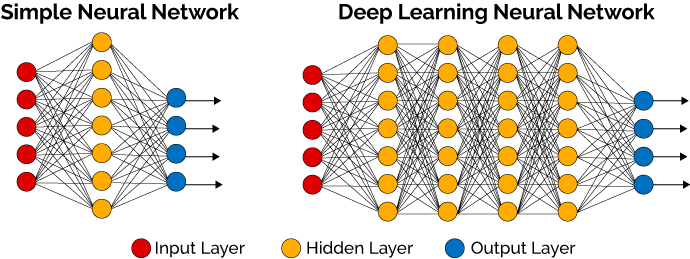
\includegraphics[width=0.77\textwidth]{Pictures/dnn.png}
    \caption{Difference between Simple Neural Network and Deep Neural Network, https://becominghuman.ai/deep-learning-made-easy-with-deep-cognition-403fbe445351}
    \label{fig:awesome_image}
\end{figure}

%	\begin{verbatim}
% 	$ vi .profile
%  \end{verbatim}


\section{Technical Keywords}\
\begin{enumerate}
    \item \textbf{\LARGE\color{ocre}Deep Learning}:  Deep learning is an aspect of artificial intelligence (AI) that is concerned with emulating the learning approach that human beings use to gain certain types of knowledge. At its simplest, deep learning can be thought of as a way to automate predictive analytics.Deep learning is the branch of machine learning which having ability to learn multiple level representation from structured data using supervised or unsupervised learning.
    \vspace{2mm}
    \item \textbf{\LARGE\color{ocre}Personalization}: Personalization goes more with the user's decisions, this means, the instructions explicitly given. An example could be the background image of twitter could be taken as personalization of your twitter profile.
    \vspace{2mm}
	\item \textbf{\LARGE\color{ocre}Online Interest}: Get users interest through social media like twitter,facebook.For that data need to mine.
	\vspace{2mm}
	\item \textbf{\LARGE\color{ocre}Social Media}: To  mine users point of interest need to get data from usesrs social account.

 \end{enumerate}

%----------------------------------------------------------------------------------------
%	CHAPTER 3
%----------------------------------------------------------------------------------------

\chapterimage{3introduction.jpg}
\chapter{Introduction}

\section{Project Idea}
\paragraph*{} Real estate appraisal, which is the process of estimating the price for real estate properties.\\
A report published by EPRA(\emph{Europian Public Real Estate Association}) real estate in all its forms accounts approximately 18-20 percent of its economical activity.therefore accurate prediction of real estete properties are crucial. For most of the working classes housing has been one of the largest expense, so to make right decision on the real estate investment is much cruicial.


\section{Motivation of the Project}  
\paragraph*{}  As we seen the report published by EPRA and why investment in  housing 
is important the thats why accurate preduction of real estate properties are crucial.Traditionally previous work for  prediction of price is based on regression analysis and machine learning.but due to rapid development in Deep Neural Network feild it is much benificial to use DNN instead of Regression.Beacuse of recently developed deep learning,computer becomes smart enough to interpret visual content in similar way that human can.\\
peoples can able to estimate price more accurately in this system as compared to previous systems only because of DNN.

\section{Literature Survey}
\begin{remark}
    J. Frew and G. Jud, “Estimating the Value of Apartment Buildings,” Journal of Real Estate Research
    \begin{itemize}
        \item Techniques : Hedonic modeling techniques to estimate
        \item Advantages : Able to estimate prices correctly in proportion of size and number of units
        \item Disadvantages : Effect of Aging isn't considered effectively
    \end{itemize}
\end{remark}

\begin{remark}
    R. E. Lowrance, “Predicting the Market Value of Single-Family Residential Real Estate,” Technical Report
    \begin{itemize}
        \item Techniques : Local Linear model and Random Forest model
        \item Advantages : lowest expected error on unseen data and model is tailored to zip codes using indicator variables
        \item Conclusion : Random forest model may perform better than the local linear model
    \end{itemize}
\end{remark}


\begin{remark}
    X. Hu and M. Zhong, “Applied Research on Real Estate Price Prediction by the Neural Network,”
    \begin{itemize}
        \item Techniques : Backpropagation neural networks and Elman neural network
        \item Advantages : Elman neural network could forecast more accurate
and constringe faster than other approaches
    \end{itemize}
\end{remark}


\begin{remark}
    N. Nguyen and A. Cripps, “Predicting Housing Value: A Comparison of Multiple Regression Analysis and Artificial Neural Networks,”
Journal of Real Estate Research
    \begin{itemize}
        \item Techniques : ANN and multiple regression analysis
        \item Advantages : when enough data points were available for training, ANNs could perform better than multiple linear regressions
    \end{itemize}
\end{remark}


\begin{remark}
    Y. E. Hamzaoui and J. A. H. Perez, “Application of Artificial Neural Networks to Predict the Selling Price in the Real Estate Valuation Process”
    \begin{itemize}
        \item Techniques : Feed-forward backpropagation neural network with a single hidden layer
        \item Advantages : reliable prediction of house selling prices at that time
    \end{itemize}
\end{remark}


\begin{remark}
    X. Zhang, “Using Fuzzy Neural Network in Real Estate Prices Prediction”
    \begin{itemize}
        \item Techniques : fuzzy neural network to support fuzzy reasoning and learning
        \item Advantages : works better than traditional neural network approaches
    \end{itemize}
\end{remark}


\begin{remark}
    S. Chopra, T. Thampy, J. Leahy, A. Caplin, and Y. LeCun, “Discovering the Hidden Structure of House Prices with a Non-Parametric Latent Manifold Model”
    \begin{itemize}
        \item Techniques : Latent Manifold Model
        \item Advantages : with two trainable components like one parametric component that predicts the “intrinsic” price of a house using its features, and the second one is a non-parametric component that calculates the desirability of the neighborhood; it performs better than pure parametric or non-parametric models
        \item Disadvantages : Fails in Rular areas
    \end{itemize}
\end{remark}


\begin{remark}
    B. J. Ford, H. Xu, and I. Valova, “A Real-Time Self-Adaptive Classifier for Identifying Suspicious Bidders in Online Auctions”
    \begin{itemize}
        \item Techniques : Neural Network model
        \item Advantages : By training the neural network with newly added structured data, so it can quickly adapt to changing trends in bidding, model is able detect suspicious bidders in online auctions
        \item Disadvantages : used structured input and learning processes, and the DNNs are fully connected
    \end{itemize}
\end{remark}


\begin{remark}
    S. Zhang, Y. Bao, P. Zhou, H. Jiang, and L. Dai, “Improving Deep Neural Networks for LVCSR Using Dropout and Shrinking Structure”
    \begin{itemize}
        \item Techniques : Specialized structured neural network
        \item Advantages : Shrinking DNN structure with hidden layers decreasing in size from a lower layer to higher layers for the purpose of reducing the model size and making the model time
efficient without affecting performance.
        \item Disadvantages : they failed to justify why shrinking DNN would not affect performance, and also there was a lack of systematic approach for the network reduction
    \end{itemize}
\end{remark}

    
%\begin{table}[h]
%  \centering
%  \begin{tabular}{ c c c c c c }
 %   \hline\hline
  %  Filter / Config. & Waveband / Central $\lambda$/ Line & Obs. Date & Comment \\
  %  \hline
 %   F225W & UV filter / 235.9 nm & 26 Aug 2009 &  UV wide\\
    
%    F336W & UV filter / 335.5 nm & 26 Aug 2009 & Str$\ddot{o}$mgren $u$\\
    
   % F373N & Narrow-Band Filter / 373.0 nm & 19 Aug 2009 & Includes \textsc{[OII]}\\
    
  %  F438W & Wide-Band Filter / 432.5 nm & 26 Aug 2009 & $B$, Johnson-Cousins set\\
    
  %  F487N & Narrow-Band Filter / 487.1 nm & 25 Aug 2009 & Includes H$\beta$\\
    
 %   F502N & Narrow-Band Filter / 501.0 nm & 26 Aug 2009 & Includes \textsc{[O III]}\\
%    
    %F657N & Narrow-Band Filter / 656.7 nm & 25 Aug 2009 & Includes %H$\alpha$+\textsc{[NII]}\\
 %   
%    F673N & Narrow-Band Filter / 676.6 nm & 20 Aug 2009 & Includes \textsc{[SII]}\\
%    
%    F814W & Wide-Band Filter / 802.4 nm & 26 Aug 2009 & $I$, Johnson-Cousins set\\
   % \hline
  %\end{tabular}
  %\caption{Summary of Observations}
 % \label{tab:uno}
%\end{table}

%-------------------------------------------------------------


%----------------------------------------------------------------------------------------
%	CHAPTER 4
%----------------------------------------------------------------------------------------
\chapterimage{problemdefscope.jpg}
\chapter{Problem Definition and Scope}

\section{Problem Statement}
\paragraph*{}
To predict the price of the real estate properties which is depends upon various factors like Infrastructure,Neighbourhood environment,House age,location etc. using \emph{Structured Deep Neural Network}.

\subsection{Goals and objectives}
\textbf{Goals}
\\The Goal of this System is to predict the price of the real estate property more precisely

\textbf{Objectives}
	
	\begin{itemize}
	\item Prediction of prices of real estate property more accurately (Using DNN).
	\item Elimination of Role of Middle Person(Agent).
	\item Assessments are not only for urban areas but also for rural areas.
\end{itemize}

\section{Major Constraints}
\begin{itemize}
\item Application should be web based.
\item Supported by any browser (mobile browser,pc browser). 
\item The information store will be an PostgreSQL database.
\end{itemize}

 
\section{Outcome}
\begin{itemize}
\item  To get the estimated price of the real estate property.
\end{itemize}

\section{Applications}
\begin{itemize}
\item Housing Investment
\item Auctions
\item Real time Valuation
\end{itemize}

\section{Hardware Resources Required}
\textbf{Developing Environment:} \\
\begin{table}[!htbp]
\begin{center}
\def\arraystretch{1.5}
  \begin{tabular}{| c | c | c | c |}
\hline
Sr. No. &	Parameter &	Minimum Requirement  \\
\hline
1 &	CPU Speed &	 2.5 GHz   \\
\hline
2 &	RAM  &	8 GB  \\
\hline 

2 &	HDD  &	1 TB  \\
\hline 

\end{tabular}
 \caption { Hardware Requirements }
 \label{tab:hreq}
\end{center}
\end{table}

\textbf{Operating Environment:} \\
\begin{table}[!htbp]
\begin{center}
\def\arraystretch{1.5}
  \begin{tabular}{| c | c | c | }
\hline
Sr. No. &	Parameter &	Minimum Requirement  \\
\hline
1 &	CPU Speed &	 800 MHz \\
\hline
2 &	RAM  & 256 MB  \\
 \hline 

 

\end{tabular}
 \caption { Hardware Requirements }
 \label{tab:hreq}
\end{center}

\end{table}

\section{Software Resources Required}
\subsection{\textbf{Developing Environment }}
\textbf{Platforms :}
\begin{enumerate}
\item Operating System: Windows 10
\item IDEs: PHP Storm,Visual Studio Code.
\item Programming Language :PHP,Python
\item Database: PostgreSQL .

\item \textbf{Tools:}\\
\begin{enumerate}
    \item Documentation: TexLive(Texworks Editor) and Overleaf(Oniline LaTeX Editor)
    \item Digram: LucidChart (Online Drawing Tool)
\end{enumerate}
\end{enumerate}

\subsection{\textbf{Operating Environment }}
Platforms : 
\begin{enumerate}
\item Operating System:Windows/Linux Based version released after 2012,Mac
\item Web Browser: Chrome version released after 2012,Microsoft EDGE,Mozilla
\end{enumerate}


%----------------------------------------------------------------------------------------
%	CHAPTER 5
%----------------------------------------------------------------------------------------
\chapterimage{pplan.jpg}
\chapter{Project Plan}

\section{Estimates}
\textbf{Agile model:}\\

\begin{figure}[h]
    \centering
    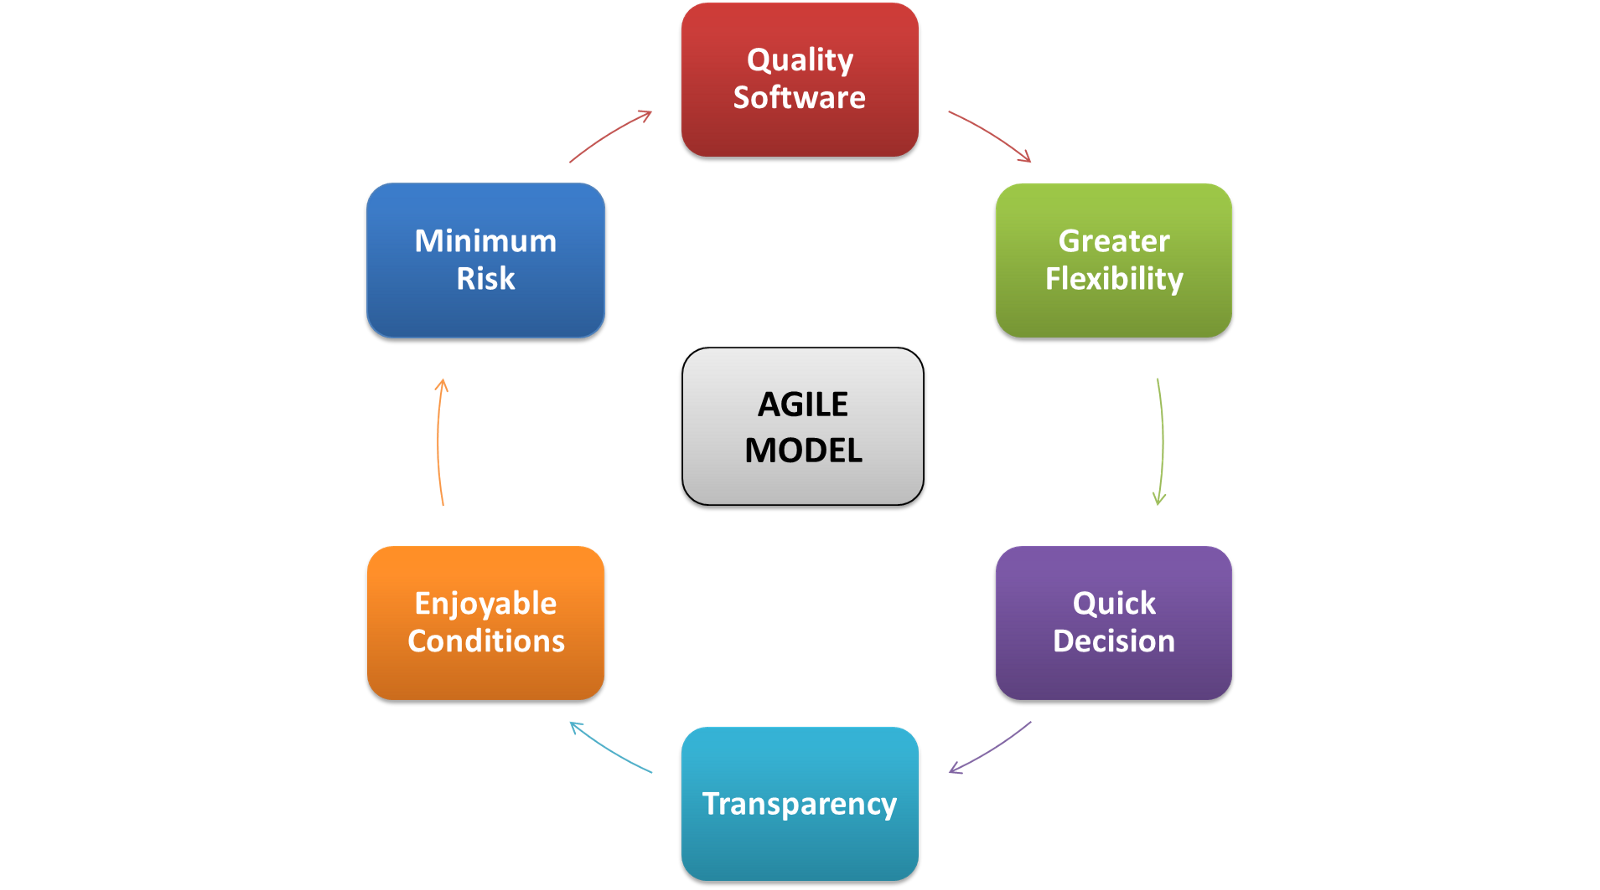
\includegraphics[scale=0.25]{Pictures/agile.png}
    \caption{Benefits of Agile Model}
    \copyright{https://medium.com/@proximitycrc/6-benefits-of-agile-model-bddf55f976b5}
    \label{fig:benefits of agile model}
\end{figure}
The Agile Method is a particular approach to project management that is utilized in software development. This method assists teams in responding to the unpredictability of constructing software. It uses incremental, iterative work sequences that are commonly known as sprints.Agile Methods break the product into small incremental builds.\textbf{Scrum} is a framework for Agile software development.

 \begin{center}
	\begin{figure}[h]
		\centering
		\fbox{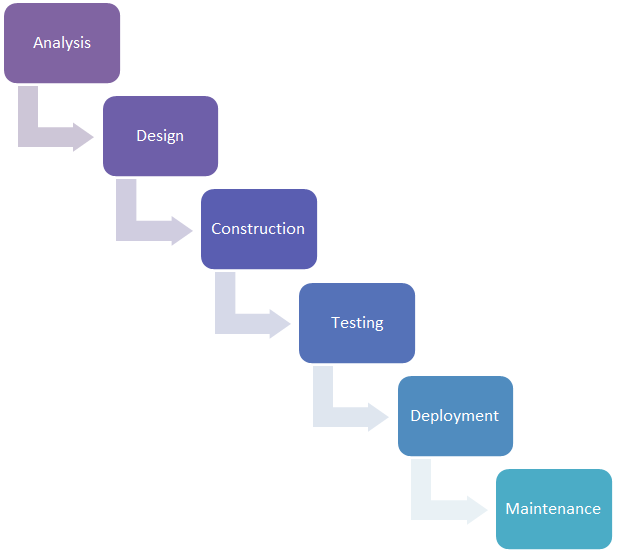
\includegraphics[scale=0.5]{Pictures/agile-development.png}}
	  \caption{Agile Model}
	  \copyright{https://www.powerobjects.com/2013/02/11/microsoft-dynamics-crm-and-agile-development}
	  \label{fig:Agile}
	\end{figure}
\end{center}

%\section{Team Organization}
%\subsection{Team structure}
%\subsection{Management reporting and communication}

%----------------------------------------------------------------------------------------
%	CHAPTER 6
%----------------------------------------------------------------------------------------
\newpage
\chapterimage{algoimg.jpg}
\chapter{Algorithms}

\section{Algorithm 1}
\subsubsection{Name}
\emph{\color{ocre}Construct Structured Knowledge}
\subsubsection{Input}
\emph{Training dataset and testing dataset in domain D}
\subsubsection{Output}
\emph{Layered Knowledge Graph (G) for domain D}
\begin{figure}[ht]
    \centering
    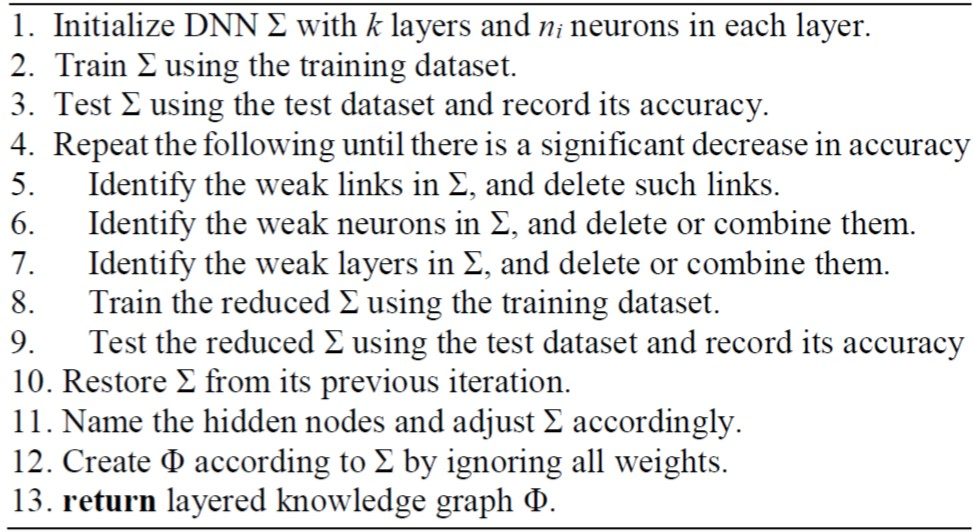
\includegraphics[scale=0.8]{Pictures/algo1.jpg}
\end{figure}
\subsubsection{Description}
\paragraph*{}
In this algorithm we take the training and testing dataset as the input and construct a Knowledge Graph from it. Firstly in this we initialize the DNN which has k layers and n(i) neurons in each layer.  Then we train DNN using the training dataset which we have taken as input. And similarly we test the DNN using the testing dataset. At this point we record its accuracy. After training and testing the DNN, we identify the weak links, weak neurons and the weak layers .So basically the weak links are the weights are the links with weak weights that are below the predefined threshold. We delete these weak links from the DNN. Then we identify weak neurons; these are the neurons with very few links, such links can also be deleted from the DNN. Or such neurons can be combined into a stronger one .After this we examine the hidden layers with very few neurons, which are called the weak layers. In a similar way we can delete the weak layer or combine two adjacent weak layers into a single one. After removal of all the outliers we again train the DNN using the training dataset and test the DNN using the testing dataset and we once again record the accuracy. We restore the resultant DNN which is a structured with no weak links or weak neurons or weak layers and we name the hidden nodes and adjust the DNN accordingly. Then we create a graph which is the layered Knowledge Graph.

\section{Algorithm 2}
\subsubsection{Name}
\emph{\color{ocre}Create Structured DNN}
\subsubsection{Input}
\emph{from algorithm 1, Layered Knowledge Graph G}
\subsubsection{Output}
\emph{a structered DNN S for Domain D}
\begin{figure}[h]
    \centering
    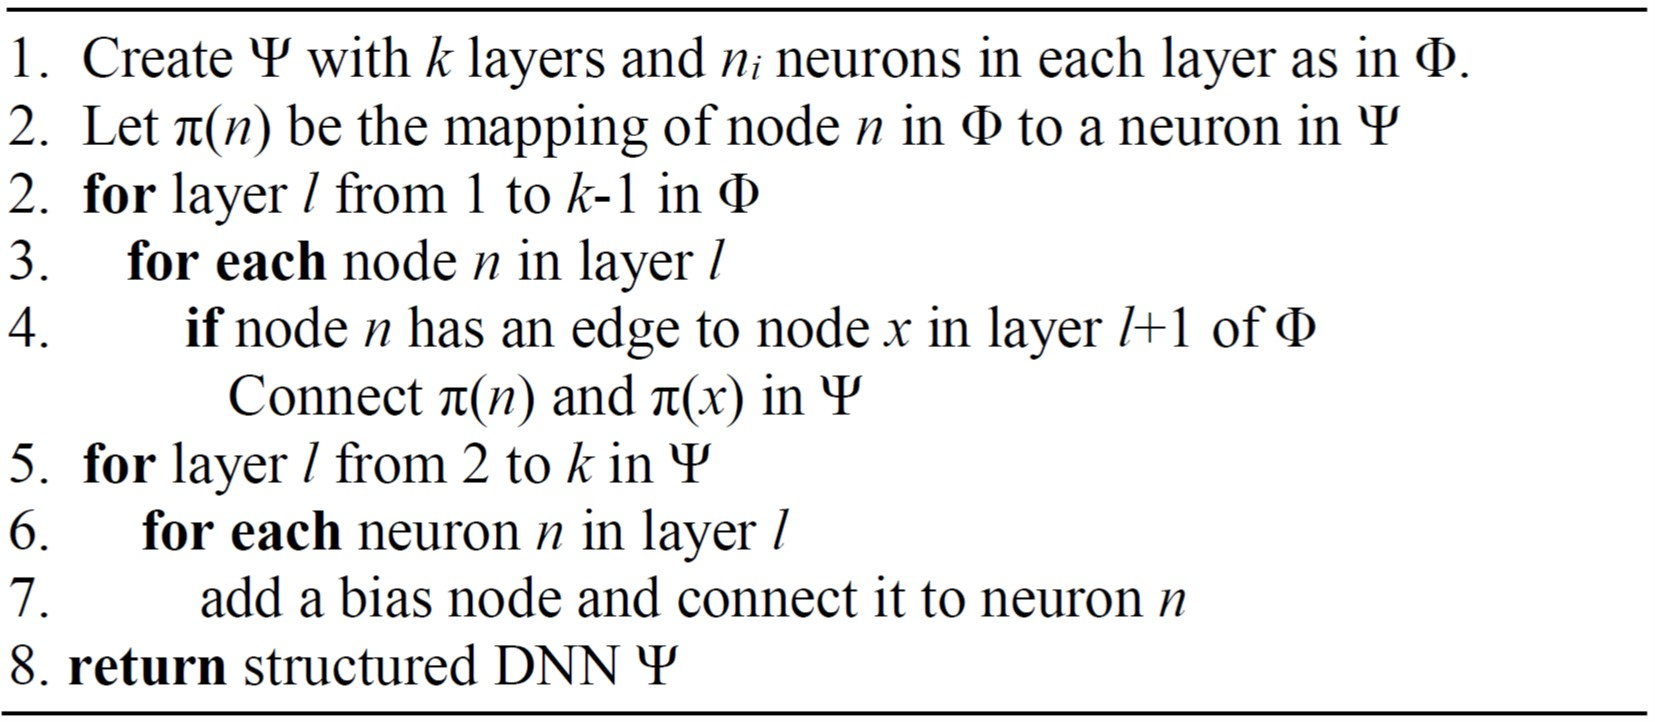
\includegraphics[scale=0.5]{Pictures/algo2.jpg}
\end{figure}
\subsubsection{Description}
\paragraph*{}
A layered knowledge graph is used to derive structured DNN it is used  for training and price prediction. Constructed DNN has 4 layers :Input layer,2 hidden layer, output layer.structured DNN trained using standard feedforward back-propagation algorithm.We initialize all connection weight with relatively small random value within range [-0.5,0.5].Structured DNN contains only needed connection between neurons,therefore it is Time and space efficient & trained using fewer data points

%----------------------------------------------------------------------------------------
%	CHAPTER 7
%----------------------------------------------------------------------------------------
\chapterimage{srs.jpg}
\chapter{Software Requirement and Specification}

%\section{Introduction}
%\subsection{Purpose and Scope of Document}
%\subsection{Overview of responsibilities of Developer}

\section{Usage Scenario}
\subsection{User profiles}
\subsubsection{Admin} Admin manage the users and also set policies.It verifies the user and provides the access rights to the System. It is able to add new Data in the model.
\subsubsection{User} User can be log in into the system and check for new places, properties and offers. They are able to add new property for sell,rent as well as for bidding.

\newpage
\subsection{Usecase Diagram}
\begingroup
\begin{center}
    \begin{figure}[!ht]
        \centering
        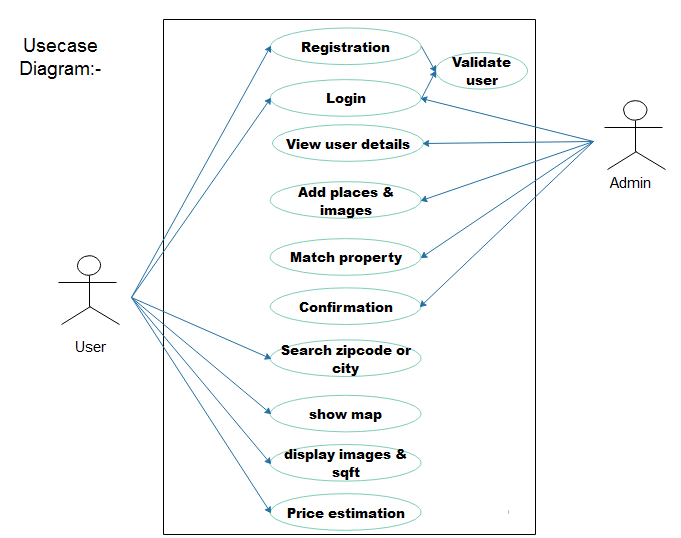
\includegraphics{Pictures/usecase.png}
        \label{fig:my_label}
    \end{figure}
\end{center}
\endgroup

%\section{Data Model and Description}
%\subsection{Data Description}

\section{Functional Model and Description}
\subsection{Data Flow Diagram}

\newpage
\subsubsection{Level 0 Data Flow Diagram}
\begin{center}
    \begin{figure}[!ht]
        \centering
        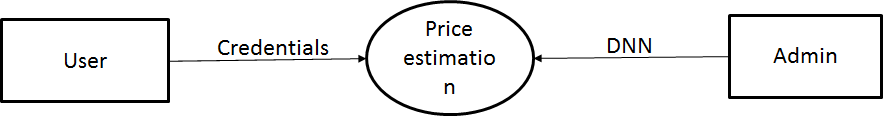
\includegraphics[scale=0.7]{Pictures/Dataflow0.png}
        \caption{Level 0 Data Flow Diagram}
        \label{fig:my_label}
    \end{figure}
\end{center}

\vspace{20mm}

\subsubsection{Level 1 Data Flow Diagram}
\begin{center}
    \begin{figure}[!ht]
        \centering
        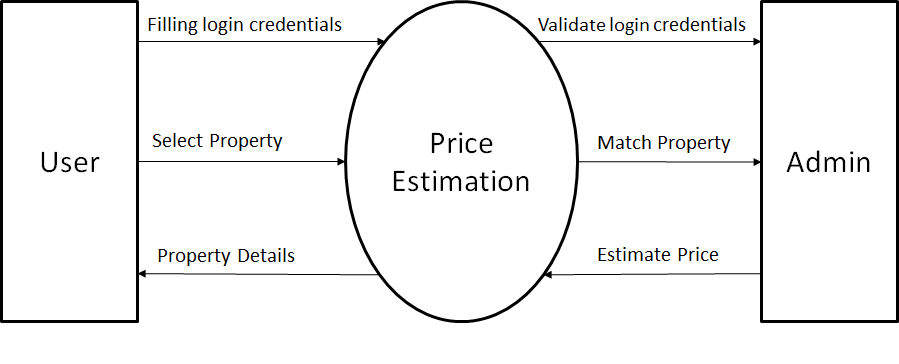
\includegraphics[scale=0.7]{Pictures/Dataflow1.png}
        \caption{Level 1 Data Flow Diagram}
        \label{fig:my_label}
    \end{figure}
\end{center}

\newpage
\subsubsection{Level 2 Data Flow Diagram}
\begin{center}
    \begin{figure}[!ht]
        \centering
        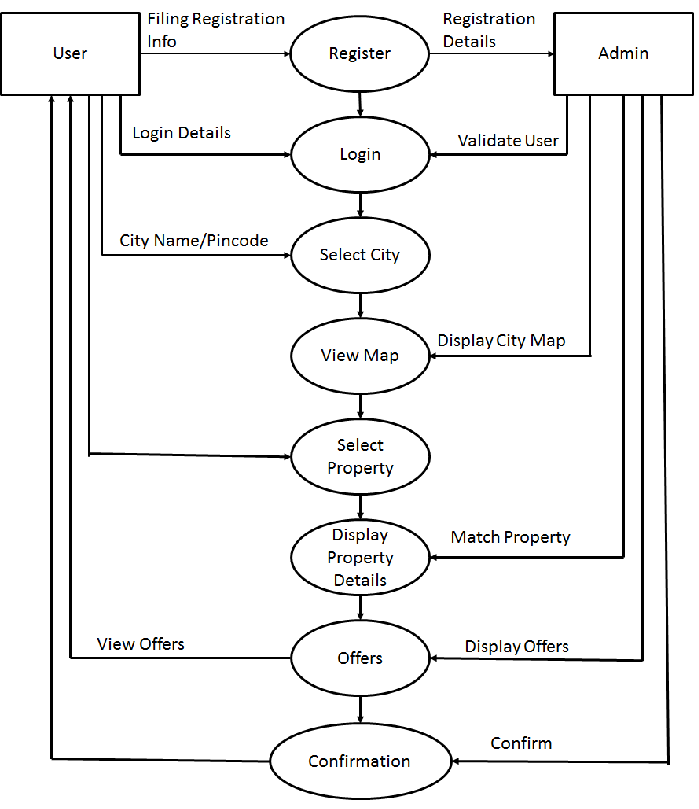
\includegraphics[scale=0.8]{Pictures/Dataflow2.png}
        \caption{Level 2 Data Flow Diagram}
        \label{fig:my_label}
    \end{figure}
\end{center}

%\subsection{Description of functions}

\newpage
\subsection{Activity Diagram}
\emph{The Activity diagram represents the steps taken.}
\begin{center}
    \begin{figure}[h]
        \centering
        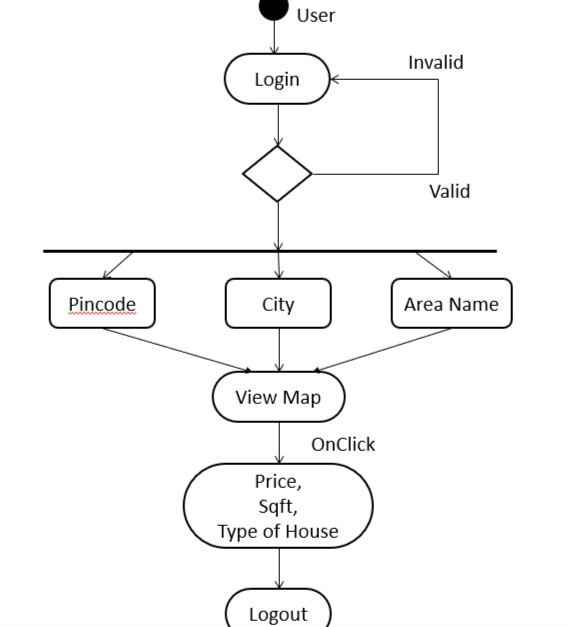
\includegraphics[scale=1.1]{Pictures/activity.jpg}
        \caption{Activity Diagram}
        \label{fig:my_label}
    \end{figure}
\end{center}

\newpage
\subsection{Non Functional Requirements:}
\subsubsection{\color{ocre}Communication interface}
It is a one-to-many user interface for communication. The users will use HTTP protocol to send queries to server.For this purpose HTML5 compatible browser is required and user can access the database through the browser by URL.
\subsubsection{\color{ocre!80}Performance Requirements}
\begin{enumerate}
\item Performance should be high i.e. response time should be low in fraction of seconds.
\item Performance is increased by providing one URL to all clients through which they can access the  database.
\item Proper updates of records database and some other information.
\item The system does not make any mistake.
\item Results needs to be shown to user in proper manner to make system effective. 
\item Appropriate colour combinations should be used.
\item The GUI must be clear,unambiguous and flexible for use.
\end{enumerate}
\subsubsection{\color{ocre}Safety Requirements}
As the database on server is centralized one there may be chances of data crash due to virus or other problems of software.So data backup is required.The record files are stored in another server and generated report files are stored on another server.Because of that no any conflict occurs.
\subsubsection{\color{ocre}Security Requirements}
Server Application is run only on the Server side, it provides Security and no chances of misuse.Proper authentication must be provided as all the data is on server.So even new admin registration must be provided only under senior admin permission .And only registered users can access the data and makes each other to their friends.
\subsubsection{Software Quality Attributes}
\begin{enumerate}
\item \textbf{Adaptability}: Any changes in software or any advanced modification will be possible.This project is reusable for creating new search engines.The algorithms used in this project can be modified in future to get more effective performance in case of reducing time and space complexity.
\item \textbf{Maintainability}: Maintains performance throughout the system.As we are providing results to query instantly within fraction of seconds it improves performance of using this search engine greatly.
\item \textbf{Portability}: System is portable to any environment. Java ,ph,python are portable and platform independent language .So main aim of using the PHP for our project is to provide portability to our project.
\item \textbf{Reliability}: Having many qualities to make system reliable.We are providing backup and recovery facility in centralize environment. This makes our database more reliable.
 \end{enumerate}
\subsubsection{\color{ocre}Database Requirements}
PostgreSQL Server  connectors are required for the connectivity between PHP and PostgreSQL server database, and php and PostgreSQL connectivity is used to store and fetch data .
\subsubsection{\color{ocre}Internalization Requirements}
To make our project global extensions required are different country languages e.g. English etc.
\subsubsection{\color{ocre}Legal Requirements}
As our project is web based project multiple users may interact with this system simultaneously with different platforms on their PC. Also our project works according to concern of user expectation. 
\subsubsection{\color{ocre}Reuse Objectives for the project}
This project can be reused in future for developing new system which provides simultaneously access .Also battery efficiency will be done because of this will be used in future for sensing  with least battery.


\subsection{State Diagram:}
Fig.\ref{fig:state-dig} example shows the \textbf{\color{ocre}State Transition Diagram}. The states are represented in ovals and state of system gets changed when certain events occur. The transitions from one state to the other are represented by arrows. The Figure below shows important states and events that occur while creating new project.
\begin{center}
	\begin{figure}[!htbp]
		\centering
		\fbox{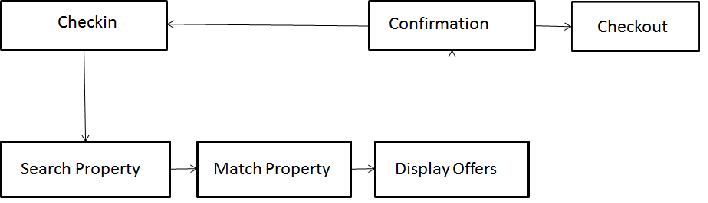
\includegraphics[width=12cm,height=10cm]{Pictures/Statediag.png}}
	  \caption{State transition diagram}
	  \label{fig:state-dig}
	\end{figure}
\end{center} 
 

 \subsection{Software Interface Description}	 
Here we will be using internet connection and HTTP protocol for web based access

%----------------------------------------------------------------------------------------
%	CHAPTER 8
%----------------------------------------------------------------------------------------
\chapterimage{chap8.jpg}
\chapter{Detailed Design Document}

\section{Introduction}  
This document specifies the design that is used to solve the problem of Product.  
\section{Architectural Design}  
	A description of the program architecture is presented. Subsystem design or Block diagram,Package Diagram,Deployment diagram with description is to be presented.

 
  \begin{center}
	\begin{figure}[!htbp]
		\centering
		\fbox{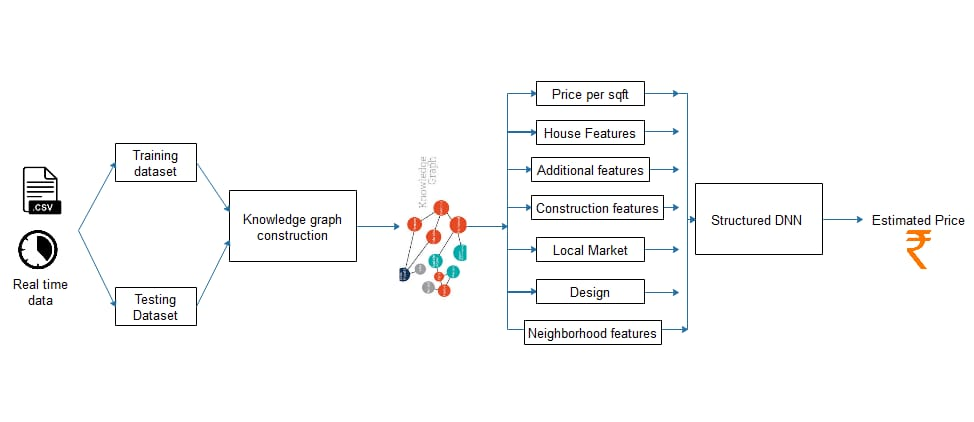
\includegraphics[scale=0.5]{Pictures/arch.jpg}}
	  \caption{Architecture diagram}
	  \label{fig:architecture diagram}
	\end{figure}
\end{center} 

\subsection{Data Collectin and Preprocessing}
We collected real estate data from a real estate website Zillow.com. This website conserves all recent and past house listings data including house features, market features, public records of houses, neighborhood features, etc. An entire number of 15 features are predefined and their associated values are collected. The predefined features include number of beds, number of baths, square footage, lot size, built year, yearly tax, similar houses average sold price, adjacent schools average ratings, fireplace, waterfront, the number of stories, heating, cooling, patio, and park. In our approach, we first remove the following outliers:  First is data points with insufficient information, e.g., missing square footage. And second is data points with unreasoning values such as a sold price of 1 as a gift. We additional calculate the average selling price of houses sold in last few months. Houses with too high or too low price-per-square feet are considered all outliers, and thus they are omitted from the training datasets and test datasets.


\subsection{Layered Knowledge Graph}
 A knowledge graph is a graph with entities of different types as nodes and several relations between them as edges. Knowledge graph aims to represent entities and the relations between entities.  We consider that a Deep Neural Network, which can produce suitable outputs with fewer weak connections between the neurons, would be nearer to a representation of a knowledge graph in a given field. We have selected a fully connected DNN with 2 hidden layers and 12 neurons in each hidden layer for our case study. In this selected neural network, the input layer contains 15 neurons, representing the predefined input features for house cost assessments, and a single output neuron representing the assessed house value or predicted selling price. We derived a layered knowledge graph for the real estate domain. We can see that the first layer contains 15 input nodes indicating that all selected features have important influences on house price assessments. The total number of hidden neurons in the second and third layer has been reduced from 12 to 10 and 7, respectively. This is due to the weak links and weak neurons being removed from the network. Finally, a single neuron in the last layer represents the assessed house value or predicted selling price
 
 
 \subsection{\color{ocre} Structured DNN}
 A deep neural network is a type of neural network in which there exist a certain level of complexity. It is a neural network with more than two layers. The structured DNN is considered to match with the knowledge graph. We made experiments on fully-connected DNNs with different numbers of hidden layers and different numbers of neurons in each hidden layer. The structured Deep Neural Network has four layers such as an input layer, two hidden layers, and an output layer. We set up suitable hyper-parameters for the structured DNN, and trained it using algorithm such as standard feed forward and back propagation algorithm with problem-specific real-time training and fitting techniques. Note that the first layer of the network contains 15 input neurons, which always produce outputs, as there are no biases are connected to the input layer neurons. Even though minor initialized weights create a neural network learn slowly, with sufficient offered data points, adjust a deep neural network with lesser weights which will help to get improved generalization, so to get good performance.



\newpage
\section{Component Design} 
\subsection{Class Diagram}
 \begin{center}
	\begin{figure}[!htbp]
		\centering
		\fbox{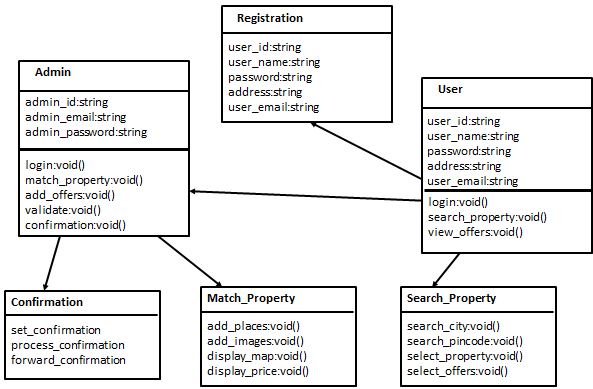
\includegraphics[scale=1.1]{Pictures/classdiag.png}}
	  \caption{Class Diagram}
	  \label{fig:class-dig}
	\end{figure}
\end{center} 
\newpage
\subsection{Sequence Diagram}
 \begin{center}
	\begin{figure}[!htbp]
		\centering
		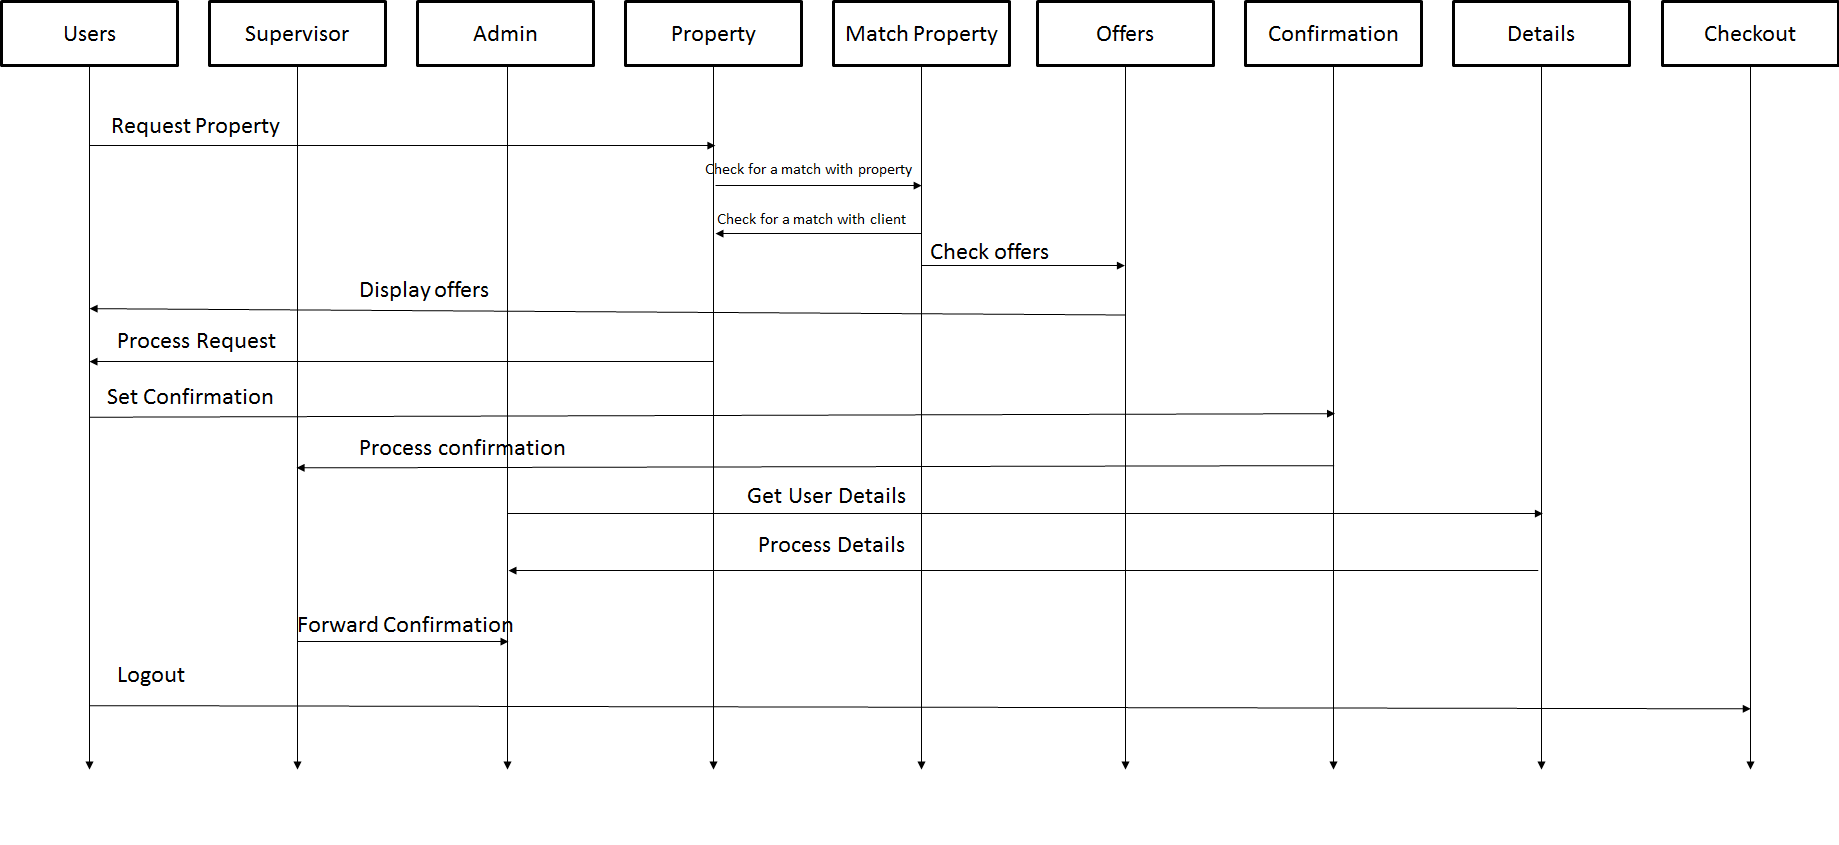
\includegraphics[width=15cm,height=15cm]{Pictures/Sequencediag.png}
	  \caption{Sequence Diagram}
	  \label{fig:seq1-dig}
	\end{figure}
\end{center}


\newpage
\subsection{Deployment Diagram}
 \begin{center}
	\begin{figure}[!htbp]
		\centering
		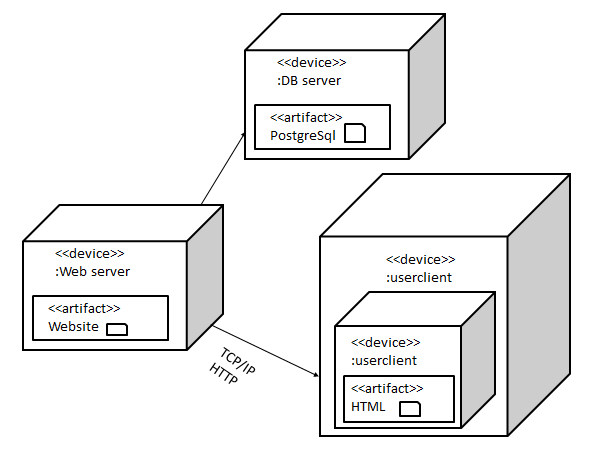
\includegraphics[width=15cm,height=15cm]{Pictures/Deployment.png}
	  \caption{Deployment Diagram}
	  \label{fig:seq1-dig}
	\end{figure}
\end{center}



%----------------------------------------------------------------------------------------
%	CHAPTER 9
%----------------------------------------------------------------------------------------

\chapterimage{conclusion.jpg}
\chapter{Conclusion and Future Scope}
\lettrine[lines=2]{\color{ocre} P}{redictive} analytic has become more and more important in the world of big data and machine learning. Here for prediction purpose we are going to use Deep Neural network instead of Regression analysis. Due to the large size of a deep learning architecture, deep learning typically requires a large amount of data to train the model, which makes the training process very time and space inefficient. In addition, a large deep architecture may also prone to have the over-fitting issue.Our experimental results given in research paper show that the proposed approach outperforms other conventional methods and leading real estate companies such as \emph{Zillow} and \emph{Redfin}, with significantly improved accuracy for house-price prediction.

\subparagraph*{}
For future research, we will study how to automate the process of extracting layered knowledge graphs from the real estate domain based on historical data, and design structured DNNs using the graphs. We will allow a DNN model to automatically change its network structure along the time, so it can be more scalable and better adapt to new market changes. Furthermore, we plan to implement our approach using mobile cloud computing. that supports assessments of real estate via mobile devices with computation functions deployed in the clouds. Finally, we will try to apply our approach to predictive analytic problems from other domains. such as stock market, health-care, transportation, marketing, e-commerce, security, business, and many more. 

%----------------------------------------------------------------------------------------
%	REFERENCES
%----------------------------------------------------------------------------------------
\newpage
\bfseries \fontsize{15}{19}\normalfont\centerline{\LARGE\color{ocre} References}
\begin{remark}
    Haiping Xu and Amol Gade, \emph{“Smart Real Estate Assessments using Structured Deep Neural Networks”} IEEE 2017, pp.255-266.
\end{remark}

\begin{remark}
    Quanzeng You, Ran Pang, Liangliang Cao, and Jiebo Luo, Fellow, IEEE
 \emph{“Image Based Appraisal of Real Estate Propertie”} in CIKM, 2017, pp. 481–490.
\end{remark}

\begin{remark}
    N. Nguyen and A. Cripps Predicting Housing Value: \emph{"A Comparison of Multiple Regression Analysis and Artificial Neural Networks,”}  Journal of Real Estate Research, vol. 22, no. 3, pp. 313-336, 2016
\end{remark}

\begin{remark}
    Y. E. Hamzaoui and J. A. H. Perez, \emph{“Application of Artificial Neural Networks to Predict the Selling Price in the Real Estate Valuation Process”} in MDM, vol. 2, 2015, pp. 31–36.
\end{remark}

\addcontentsline{toc}{section}{References}

%----------------------------------------------------------------------------------------
%	Group Members
%----------------------------------------------------------------------------------------
\newpage
\begingroup
\thispagestyle{empty}
\AddToShipoutPicture*{\put(0,0){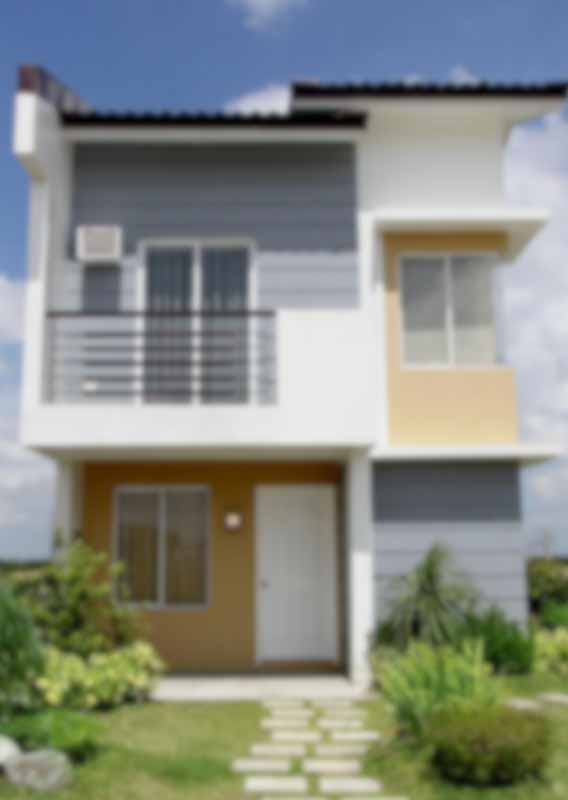
\includegraphics[scale=1.25]{aboutus_edited.jpg}}} % Image background
\centering
\vspace*{2cm}
\par\normalfont\fontsize{40}{35}\sffamily\selectfont

\vspace*{4cm}
\textbf{Information of Project Group Members}\\ % Project title
\vspace*{4cm}
\endgroup
\addcontentsline{toc}{section}{About Us}

%------------------------------------------------------------------------------------------
\newpage
\begin{figure}[h] %this figure will be at the right
    \hspace{100mm}
    
\includegraphics[width=0.25\textwidth]{Pictures/pgsql.png}
\end{figure}
\begin{enumerate}
\begingroup
\thispagestyle{empty}
\AddToShipoutPicture*{\put(0,0){
\includegraphics[scale=1.25]{Pictures/pink_gradient_5k-7680x4320_edited.jpg}}} % Image background
\par\normalfont\fontsize{20}{15}\sffamily\selectfont\color{white}

\vspace*{2cm}
    \item Name : Patne Nikhil Sunil\\[0.5cm]
    \item Date of Birth : 29/10/1997\\[0.5cm]
    \item Gender : Male\\[0.5cm] 
    \item Permanent Address : A/p Dhom, Tal.-Wai, Dist.-Satara\\[0.5cm]
    \item E-Mail : nikhilpatne94@gmail.com\\[0.5cm]
    \item Mobile : 8605358076
\end{enumerate}
\endgroup

%------------------------------------------------------------------------------------------
\newpage
\begin{enumerate}
\begingroup
\thispagestyle{empty}
\AddToShipoutPicture*{\put(0,0){
\includegraphics[scale=1.25]{Pictures/pink_gradient_5k-7680x4320_edited.jpg}}} % Image background
\par\normalfont\fontsize{20}{15}\sffamily\selectfont\color{white}
\vspace*{2cm}
    \item Name : Shinde Abhishek Sunil\\[0.5cm]
    \item Date of Birth : 14/03/1997\\[0.5cm]
    \item Gender : Male\\[0.5cm] 
    \item Permanent Address : A/p Phaltan, Tal.-Phaltan, Dist.-Satara\\[0.5cm]
    \item E-Mail : shindea890@gmail.com\\[0.5cm]
    \item Mobile : 7276643616
\end{enumerate}
\endgroup

%------------------------------------------------------------------------------------------
\newpage
\begin{enumerate}
\begingroup
\thispagestyle{empty}
\AddToShipoutPicture*{\put(0,0){
\includegraphics[scale=1.25]{Pictures/pink_gradient_5k-7680x4320_edited.jpg}}} % Image background
\par\normalfont\fontsize{20}{15}\sffamily\selectfont\color{white}
\vspace*{2cm}
    \item Name : Gholap Satyawan Ashok\\[0.5cm]
    \item Date of Birth : 02/10/1996\\[0.5cm]
    \item Gender : Male\\[0.5cm] 
    \item Permanent Address : A/p Varand, Tal.-Daund, Dist.-Pune\\[0.5cm]
    \item E-Mail : satyawanraje7@gmail.com\\[0.5cm]
    \item Mobile : 9561522780
\end{enumerate}
\endgroup

%------------------------------------------------------------------------------------------
\newpage
\begin{enumerate}
\begingroup
\thispagestyle{empty}
\AddToShipoutPicture*{\put(0,0){
\includegraphics[scale=1.25]{Pictures/pink_gradient_5k-7680x4320_edited.jpg}}} % Image background
\par\normalfont\fontsize{20}{15}\sffamily\selectfont\color{white}
\vspace*{2cm}
    \item Name : Dange Namrata Milind\\[0.5cm]
    \item Date of Birth : 08/05/1998\\[0.5cm]
    \item Gender : Female\\[0.5cm] 
    \item Permanent Address : A/p Junction, Tal.-Indapur, Dist.-Pune\\[0.5cm]
    \item E-Mail : dangenm@gmail.com\\[0.5cm]
    \item Mobile : 8600551630
\end{enumerate}
\endgroup

%------------------------------------------------------------------------------------------
\newpage
\begin{enumerate}
\begingroup
\thispagestyle{empty}
\AddToShipoutPicture*{\put(0,0){
\includegraphics[scale=1.25]{Pictures/pink_gradient_5k-7680x4320_edited.jpg}}} % Image background
\par\normalfont\fontsize{20}{15}\sffamily\selectfont\color{white}
\vspace*{2cm}
    \item Name : Beera Vivechana Ramesh\\[0.5cm]
    \item Date of Birth : 26/01/1995\\[0.5cm]
    \item Gender : Female\\[0.5cm] 
    \item Permanent Address : A/p Baramati, Dist.-Pune\\[0.5cm]
    \item E-Mail : vivechanab5@gmail.com\\[0.5cm]
    \item Mobile : 9823838097
\end{enumerate}
\endgroup
%------------------------------------------------------------------------------------------

\end{document}